\documentclass[a4paper, 12pt]{report}

% Encoding so åäö as input, | and ascii as output, and english works as intended
\usepackage[T1]{fontenc}
\usepackage[utf8]{inputenc}
\usepackage[english]{babel}

%% Numbered citations
\usepackage[numbers]{natbib}
%% For figures
\usepackage{graphicx}
\usepackage{float}
\usepackage{subcaption} % For side-by-side figures
%% internal PDF links
\usepackage{hyperref}
%% For appending pdfs
\usepackage{pdfpages}
%% For math
\usepackage{amsmath}
\usepackage{siunitx} % Units in equations
%% For eps on windows
\usepackage{epstopdf}
%% For nice tabels
\usepackage{booktabs}

%% To make chaptertitles behave
\usepackage{titlesec, color}
\definecolor{gray75}{gray}{0.75}
\newcommand{\hsp}{\hspace{20pt}}
\titleformat{\chapter}[hang]{\Huge\bfseries}{\thechapter\hsp\textcolor{gray75}{|}\hsp}{0pt}{\Huge\bfseries}

\begin{document}
\pagenumbering{roman}

\begin{titlepage}
	\centering
	%\includegraphics[width=0.3\textwidth]{550x418.jpg}\par\vspace{1cm}
	{\scshape Kungliga Tekniska Högskolan \par}
	\vspace{2cm}
    {\huge\bfseries Eco Cars\par}
	\vspace{0.5cm}
	{\scshape\Large Elba 2016\par}
	\vspace{1.5cm}
	\begin{figure}[H]
    \centering\label{fig:ECO}
    \includegraphics[width=0.5\textwidth]{./img/ECOCARS}
\end{figure}

    {\Large\itshape{Sanel Ferhatovic, Andreas Fröderberg, Emil Hjelm, Adam Lang,
    Richard Odell, Alexander Ramm \par}}
	\vfill
	\vfill

% Bottom of the page
	{\large \today\par}
\end{titlepage}


\begin{abstract}
A hybrid vehicle, built to compete in Shell Eco-Marathon, was upgraded and modified to run on ethanol. In addition an optimal speed trajectory controller where designed and implemented to minimize energy consumption.
A roling highway, or a test rig, where designed and constructed to be able to test the cars performance on any, simulated, track's high-profile. 
The theoretical performance was evaluated, which estimated that the car would have a mileage of 197 km/litre ethanol if run on the competition track.
\end{abstract}
\clearpage
% Hardcoded page number start
\setcounter{page}{3}
\chapter*{Preface}
\addcontentsline{toc}{chapter}{Preface}
Without a few key-persons this project would never have been possible, and not
as successful. The entire experience has been great and we have learned more
than we could ever imagine.  We would first and foremost like to thank Mikael Hellgren for
being the driving force behind KTH Eco Cars, and also Lei Feng for supervising the
project and for making the optimization possible.  The team would also like to
thank the other groups within the project who made large contributions to the car before the
competition, and managing to almost get the car to complete an attempt.  There
are more people who also contributed knowledge and helped in one way or another,
both from ITRL and the Mechatronics institution.  Naturally many people are
involved in a big project like this and being a part and directing it is
something we will never forget.

\begin{flushright}Mechatronics team \\ The bunker \\This year: fore sure \end{flushright}

\clearpage
\setcounter{tocdepth}{1}
\tableofcontents

\chapter*{Abbreviations}
\addcontentsline{toc}{chapter}{Abbreviations}
\noindent{}\begin{tabular}{r  l}
\textbf{Abbreviation} 	& \textbf{Description} \vspace{.5em} \\
BLDC	&Brushless Direct Current\\
CAN	&Controller Area Network\\
CEP     &Circular Error Probable\\
DC	&Direct Current\\
GUI     &Graphical User Interface\\
HEV     &Hybrid Electrical Vehicle\\
ICE 	&Internal Combustion Engine\\
ITRL    &Integrated Transport Research Lab\\
MBD     &Model Based Development\\
SEM	&Shell Eco-marathon\\
TLC	&Target Language Compiler\\
UCV     &Urban Concept Vehicle

\end{tabular}

\clearpage
\pagenumbering{arabic}

%% The first line in the included files should be \chaper{chaptername}
\chapter{Introduction}
\section{But why}
\section{Requirement engineering}
% Written by Andreas
In a complex system, there are many stakeholders, both internal and external.
The requirements are meant to capture the needs of the users and convey them to
the developers \cite{ibm_req}. It is important that the requirements are
unambiguous \cite{ibm_req, rupp2014}. Since natural language is ambiguous by
nature, there are framewortks and templates to improve the quality of the
requirements \cite{rupp2014}. 

\subsection{User and system requirements}
Requirements can be organized into two categories, User and System requirements.
These differ in a number of ways, both in their nature and how they are
procured.

A project design starts with a need from a customer or user. These needs set the
goal of the project and are of a high level, abstract nature. They are captured
from the future users of the system and are expressed in the users language. In
essence, the User requirements describe the problem that is to be solved by the
system \cite{ibm_req}. 

When the User requirements are set, they need to be condensed into technical
requirements that the developers can work towards. These are the System
requirements. They define what the system and its sub-systems do. It is the
deveoplers that own these requirements and they are responsible that these in
turn fulfill the User requirements \cite{ibm_req}.

\subsection{Requirement formulation}
It is important that requirements are clear and unambiguous. By using templates
when expressing the requirements, there is a framework where it is agreed what a
word/phrase means. This greatly increases the quality of the requirements
\cite{rupp2014}. By using a template for the structure of a requirement, it is
ensured that all parts needed are in the requirement. Rupp \cite{rupp2014}
gives a template on how to formulate a requirement \ref{fig:req_template}.

\begin{figure}[H]
    \centering
    \includegraphics[width=\textwidth]{./img/introduction_req_template}
    \label{fig:req_template}
    \caption{Requirement formulation template.}
\end{figure}

To convey the relevant information, each requirement needs some metadata
connected to it. Thses metadata makes it possible to see the cicumstances under
which the requirement was set and will be tested, who is responsible and when
changes are made. These attributes allow requirements to be grouped and searched
\cite{ibm_req}.

In \cite{ibm_req}, a number of relevant metadata attributes are provided.
Together these make up a comprehensive view of each requirement. Since the Eco
Cars project is of medium size, attributes related to subsystems are not needed
since there are not many layers in the system architecture. In the project, the
requirement attributes that are used are displayed in Table~\ref{tab:req_attr}.

\begin{figure}[H]
    \centering
    \label{tab:req_attr}
    \caption{Requirement attributes used in the Eco Cars project.}
    \begin{tabular}{r | l }
        \bf{Status} & Stage in acceptation process. \\
        \hline
        \bf{Author} & Requirement author. \\
        \hline
        \bf{Created date} & Date when requirement was proposed. \\
        \hline
        \bf{Latest change by} & Last person that made changes to requirement. \\
        \hline
        \bf{Latest change date} & Date when requirement was last changed. \\
        \hline
        \bf{Dependencies} & Requirements that this depends on. \\
        \hline
        \bf{Requirement} & Natural language formulation of requirement. \\
        \hline
        \bf{Comment} & Signed comment to each change made.
    \end{tabular}
\end{figure}

\subsection{Requirement software}
In a complex system, there are many relationships between stakeholders and
requirements \cite{ibm_req}. Since requirements are the result of a process
where a large problem is divided into smaller parts, a change in one requirement
may affect several other requirements. Therefore, it is important to have a
requirement software that makes it easy to track the dependencies between the
different requirements \cite{ibm_req}. It is also important that it is easy for
the user to see, edit and create new requirements.

There are a number of Requirement Engineering programs available, such as IBM
Rational Doors, Siemens Polarion and RequisitePro. These all provide solutions
for creating, managing and tracking requirements in projects. All of these can
be used under paid licenses. Of these, only Doors is available to use for the
Eco Cars team since a license is provided by KTH. Doors is very full featured
and the group have some use experience from previous courses. 

The features required in this project are the requirement organization, inter
requirement tracking and test case linkning. These are part of the core set of
functionalities of Doors, there are many more features that can be used. The
redundancy of features clutters the UI and makes the program less easy to use.
Because of this, an alternative solution was chosen. The goal of this
requirements solution was to have a clean, easy to use UI that only implements
the features that are needed in the project, but at the same time was
extensible so that additional features could easily be added as needed.

The chosen implementation was an html document made with
Markdown(http://daringfireball.com). Markdown is a language that uses simple
syntax to create Markdown files (file extension .md) that are then parsed
into standard HTML. The HTML implementation allowed for linking of requirements,
both internally in the document but also externally to files in the project
folder structure using the HTML anchor-tag (<a>). To simplify the creation of
new requirements, a HTML/CSS/JavaScript local web page was created. This web
page allows the user to create syntactically correct requirements according to
the standard set by the team using a graphical UI. Using an automated solution
to generate requirement code reduces the risk of errors and makes the process of
creating new requirements less tedious and more intuitive. Should the
requirement standard format be changes, for example by adding an attribute, the
script can easily be updated and new requirements will follow the standard.

\subsubsection{Requirement format and Markdown}
Markdown uses a simple syntax to edit and typeset documents. The Markdown
document is parsed into HTML (sometimes with additional styling in CSS) using a
parser program. There are a variety of free parsers. A full reference to the
Markdown syntax is available on the home page of the language but the relevant
elements are given in {\bf appendix}. %% This needs to be added to an appendix
%% and referenced to this // AF
%% TODO: Continue the section detailing what the format of the requirements is
%% what they look like in markdown.


\chapter{Purpose}

Why is is this project even interesting?

Lowering fuel consumption is one of the main challenges for the automotive 
industry. Regularly new standards for permitted emissions are passed and  
one solution is to burn less fuel, which results in less emissions.

Hybrid vehicles have been growing in popularity over the last decade and 
more lately have the plug in hybrids emerged. These cars allows one 
to charge the car with electrical energy at home, potentially at a low price.

Elba can be called a plug in hybrid and reducing fuel (and energy) consumption is the goal
of SEM\@. But since the style of hybrid is very unique, with the triple motor/ engine
combination, the problem of reducing the fuel consumption is not trivial. 

\section{The Problem}
When driving any car around a track some parameters and variables have a large effect of
how much energy is used to propel the car forwards. Speed, weight, drag and friction are
the first that comes into mind. Both drag and friction are increased with speed.

\section{Applications}

\section{Wall of text}
If one wishes to perform well in Shell Eco-Marathon optimising the speed the car should have on the track could improve performance. 
This is also something that is interesting for the industry and is not use in current cars when using autimatic speed thingys. This would both save money and the environment due to the reduced fuel consumption.

One goal the optimisation is to improve result at SEM. Therefore a car, in competition shape, has to be maintained. The car has to be updated to comply whit the current SEM-rules and also simply to be cemt in a drivable state. The car is also seen as a platform for students to test ideas and perform research. Various parts of the car have already been developed as bachelors thesis's and the optimisation will be improved as a part of a master thesis. The car enables students to try to solve both complex construction and design tasks, such as the unique clutch or the laminate door, and experiment with different optimisation strategies in a real world case. Appearing and performing well with the car is the main way to get sponsorship deals to support the project, both with parts and with money to cover travel and transportation costs.

But to be able to do all this test has to be carried out with as little overhead(time, track, transportation etc.) as possible. Also the actual competition track is located in London (and it only exists during the event), so there is no option to go there and test. This is the motivation behind the testrig. Other teams competing in SEM uses these machines to test the car while standing still, but KTH EcoCars had no machine like this. The testrig solves several practicalities for KTH EcoCArs and is therefore not only benificial for the car that was worked on, Several problems had to be solved for it to work: is must supply the torque demanded, is must simulate the forces the car is exposed to, and is has to handle supply of energy and regenerated energy created when braking the car.
\chapter{Elba The Car}
The hybrid vehicle that was build upon was named Elba several years ago when it
was still a pure electric vehicle. The platform has been continuously improved
and altered to the complex hybrid that exist today. Each year Elba participates
in Shell Eco Marathon (SEM) as an ``Urban Concept Vehicle''.

%Introduction
\section{Introduction}
This section gives an introduction to Elba
\subsection{Propulsion}
Elba is an electric-ethanol hybrid vehicle which combines two 48V electrical
motors and one internal combustion engine (ICE). The electrical motors is one
0.2 kW direct current (DC) motor connected directly to the drive shaft and one
1.1 kW brushless DC motor (BLDC) connected via the clutch to the drive shaft.
The one-cylinder four-stroke ethanol powered ICE is connected to the drive
shaft via the clutch. These three provide a driving torque to the rear drive
shaft. The drive shaft is then connected to the right rear wheel via an 1:10
ratio planetary gear. The car fits a single human, he or she is also the
driver. The driver steers the car manually and decides upon a reference speed
that the car should follow and has the option to decides what motor/engine
combination that should be used at a specific time.

\subsection{Aim}
The aim of Elba is to provide a research platform to perform various levels of
projects for students from different science fields, while at the same time be
accepted to compete in SEM\@. The projects can vary in time and
extent and can be independent or made as an long term implementation. 

\subsection{Shell Eco-Marathon}
SEM is a vehicle competition focused on fuel efficiency where engineering
students from around the world designs, builds and drives their own vehicles.
The competition is split into two classes. The Prototype class is solely
focused on fuel-efficiency and have less restrictions concerning comfort and
usability compared to the second class which is the UrbanConcept class,
see~\ref{UCV}.

\subsection{Urban Concept Vehicle}\label{UCV}
ELBA competes in the UrbanConcept class and is what is called a UrbanConcept
Vehicle (UCV). The vehicles in this class have an appearance closer to today's
production type passenger cars. The cars in the class have to be built in
accordance with the class specific rules that dictates everything from steering
and controls to propulsion and safety. UCVs must have some common production
car features as wind shield wiper, turn signals, horn headlights etc. Vehicles
competing in this group is also required ``stop and go'' each lap, which means
that once every lap the vehicle needs to do a full stop. This is to further
increase the resemblance to city driving.

\subsection{State at start of project}
The car where in working condition when the project started, but had several
problems. To mention a few major ones: The clutch where slow and unreliable,
the overall power-output might not have been enough to be efficient on the new
track, none of the potential driver would fit in the driver compartment, the
horn disturbed the entire electrical system.

These issues where, together with the competition rules, the primary base for
the decisions that where taken and related to the car. Some of the work done to
``fix'' these problems where a matter of reshape some metal piece and bolting it
back in the car, suddenly the driver could reach the brakes. While other
required an entire team of people to get a new, working, ethanol engine in the
car.

%System Overview
\section{System Overview}
\subsection{Electronic Control Units}
The car has four electronic control units (ECUs) that are responsible for
controlling different parts of the car.

\begin{itemize}
\item Front-ECU
\item Back-ECU
\item ICE-ECU
\item Clutch-ECU
\end{itemize}

The Front-ECU is responsible for the human interface, the buttons where the
driver is able to decide mode and speed if the car is in manual mode. It sends
speed and dive mode on the can bus.

The Back-ECU controls the motors via the separate motor controllers. It has
veto over the ICE and Cluch.

The internal combustion engine is controlled by the ICE-ECU and this is its
only task. It senses the lambda value and motor? temperatures to control the
injection of fuel.

The Cluch-ECU controls the clutch. It interfaces to two H-bridges which in turn
steers the linear actuators.  

\subsection{Communication}
The car uses a CAN network to communicate between the distributed
micro-controllers. The micro-controllers have specific values that are needed
elsewhere; these are sent on the CAN-bus. 

Another CAN network is used between the Back-ECU and the inMotion driver that
controls the brushless motor. This newtwork ustes the protocol CANopen that
lies on top of the CAN bus.
The instrumentation panel communicates via Bluetooth with the data-logger/GPS-unit.

\subsection{Energy supply}
All energy used to propel the car forwards (during the competition) comes from
the ethanol fuel, but electrical energy can be stored in the super-capacitor.
When the electrical motors generate energy it can be stored in this
super-capacitor for later use. The car can only start from standstill using one
of the electrical motors with energy from the super-capacitor.  


\section{Software and Simulation Models}
Using a model based approach relies on verified systems models on various levels. Elba benefits form a full system model to simulate fuel efficency and each ECU has a corresponding simulink model from which all code is compiled. 
\subsection{Plant Model}
The plant model is supposed to be a full system model capable of estimating fuel consumption over an entire SEM attempt. When any component, which has an affect on propulsion, is changed on the car the plant model must also be updated. Naturally the goal with MBD is that any change can be simulated with the plant model, approved and then the car is updated. But not all simulations can be done beforehand, which was the case for the new ICE.\@

\subsection{ECU software}
All ECUs use an Arduino (Due or Mega) as micro-controller which simulink has
compiler support for. This means that simulink models can be compiled and
uploaded to the arduino directly from simulink. The Simulink to Arduino coupling also
gives the option for running ``external mode'' a Hardware in the loop type compile mode.
This makes it possible to look at values and signals, running on the ECU, in
real-time.
 
%Requirements
\section{Requirements}
\subsection{Rules}
At Shell Eco Marathon all vehicles must pass two inspections before the vehicle is allowed to enter the track. First a safety inspection evaluating if it's dangerous to have the vehicle on the track, both for the driver and other vehicles. And second a technical inspection asserting if the vehicle complies with the competition rules.

%Design Decisions
\section{Design decisions}
\subsection{Clutch decisions}
%1. What the old team told us
%2. What we told MD to do
%3. What MD did
%4. Problems still
%5. Finding the problem
%6 Fixing the arms

One of the major problems with the car has been the clutch. Figure(\ref{fig:Drivetrain}) illustrates the mechanical components of the drivetrain of elba.

\begin{figure}[H]
    \centering
    \label{fig:Drivetrain}
    \includegraphics[width=1\textwidth]{./img/Drivetrain}
    \caption{Illustration of the mechanical components of the clutch, where the red plates can move towards the center plate to engage and disengage the motors to the drive shaft.}
\end{figure}

The Problem stated when starting the project was that the clutch actuators were oversized and thus giving more force than necessary for the clutch to engage properly. When the clutch was engaged with too much force, the clutch plate on the ICE side stuck very hard to the center plate and could not be disengaged using the actuator.

To solve the mechanical problems it was decided to appoint one team from the machine design department to work solely on the mechanical parts of the clutch. The mechatronics team decided to completely remake the clutch ECU to make it more robust. Despite the new ECU and the work performed by the machine design team, which can be read about in (TODO REPORT.XX) there was problems with the clutch when it was time to race. The problems was of the same mechanical nature as before the rework, where the clutch plate on the ICE side could not be disengaged from the drivetrain.

To solve this problem, several solutions have been investigated. The clutch mechanism has been controlled by time rather than position. One approach was to use the built in hall sensor in the actuator to control the position. One other idea was to use an external current sensor on the clutch ECU to control the position. A third idea was to continue using time as reference, but increase it so that an end position is always reached, which can be used as a reference position.

When investigating alternative three above using longer time to engage and disengage the clutch a new problem was discovered. It appeared that even though the clutch was not stuck to the center plate it still could not be properly disengaded. This was due to the geometry of the lever arm which pushes the clutch plate.  After this important insight the drivetrain was disassembled and new lever arms were constructed and manufactured. When the drivetrain was assembled again the clucth worked like a charm. Figure(\ref{fig:clutch}) is a rendered image of one of the new lever arms.

%%TODO
\begin{figure}[H]
    \centering
    \label{fig:clutch}
    \includegraphics[width=1\textwidth]{./img/clutch}
    \caption{The new clutch lever arms}
\end{figure}


\subsection{Internal Combustion Engine and ICE ECU}
It was decided that this years car should compete in the alternative fuels
class. This means that the car should be powered by an engine that runs on
ethanol. An engine running ethanol need to have a higher compression ratio than
a petrol engine.
%% TODO: Source on the above. Also, link to ICE report.
The requirements engineering and modifications on the new ICE was set by the ICE
team. To control the new engine, a new ICE ECU was needed. It was also decided
that the new ICE ECU would contain more sensor inputs as well as the possibility
to control the ICE ignition. All functionality of the old ICE ECU would still be
present, namely:
\begin{itemize}
    \item Simulink TLC software.
    \item Feedback control loop of injection time.
    \item Lambda value sensing.
    \item Encoder reading with index pulse from ICE\@.
\end{itemize}
More sensor data together with ignition control would give possibilities
for more exact control of the ICE\@. The extra features of the new ECU were:
\begin{itemize}
    \item Motor oil temperature sensing.
    \item Ambient air temperature sensing.
    \item Ignition control.
\end{itemize}
The features were implemented on the ECU PCB and the system was designed so that
the sensors and features could be implemented incrementally according to the
time and need of the project. Given that the amount of time that would be needed
to get the car in working condition before the race was not easily planned
beforehand, it was beneficial to have a base functionality with flexibility to
add features.

\subsection{Door}
The car is required to have a door, with a large enough entrance and working locking mechanism \cite{semrules16c1}. Since the old, layered carbonfibre door was too flimsy and also back hinged (there is a reason its call "suicide door"), it was decided a new, sturdier, door would be made. Two lightweight-construction student took this upon them self as a bachelors project. 

The new door where constructed in a carbon fibre sandwich style and was open in a scissor manner. The door became sturdier but the hinges where less than ideal and the closing mechanism did not work.

%Results
\section{Results}
We beat Chalmers. We are no byskola.
\subsection{Competition}
At the time the team arrived in London the ICE had never been started with only ethanol as fuel, the door had to be mounted and an number of small changes to be able to pass both inspections. Most time where spent to get the engine running, but it was never able to run for more than a couple of strokes. 

Both the technical inspection and safety inspection were passed. There where a few complaints: The doors closing mechanism where insufficient, the indicator lights where to weak, and the fire-extinguishers expirations data had passed. All these had to be reinspected before ElBa where given a pass.

It was decided that one attempt should be made even if the engine never had been started properly. Since the car must be rolling to start the ICE the inertia of the car will keep the ICE turning even if it misfires (the wheel inertia is no enough for this). This meant that the ICE started once the car finally was running during the attempt. But it was soon discovered that the engine could not be shut off, if the clutch was disengaged the engine kept running and revving at dangerous levels. Since the car is required to stop once each lap ElBa had to stall the engine with clutch engaged. While trying to get going again the clutch could not be disengaged and the attempt had to be aborted.

Therefore ElBa never got an competition result. But many lessons where learned.

\subsection{End of project}

\section{Conclusion}

\chapter{Optimization}
\section{Introduction}
The main goal of the project is to have the car consume the least amount of fuel
possible. In the ideal world should the engines and motors therefore always operate
within a certain the range of their optimal point of operation. The torque request
from each of the engine/motors should be with this goal in mind in order to reduce
fuel consumption. In addition to this goal, there is a number of constraints that
needs to be considered on top of this generic optimization.  Things like track
topography, super-capacitor voltage, competitors on the track etc will all weigh in
on the output request. The optimization algorithm used ELBA was developed as a part
of a Master Thesis~\cite{lui2016}. The control architecture for ELBA consists of a
two or three layers and the thesis have completed the top layer speed reference
control. This chapter will cover the decentralized hierarchical predictive control
that is used to calculate the speed trajectory.

\section{Constraints}
The optimization is limited by the constraints of the physical system, meaning that
the controller is not able to operate outside the limits of the system. These limits
are,
\begin{align}
    &U_{cap} \in [39,48]~\textup{V} \\
    &\nu \in [0,15]~\textup{m/s}\\
    &a_{max} \in [-1,1]~\textup{m/s$^2$}
\end{align}
where $U_{cap}$ is the voltage level of the super-capacitor, $\nu$ is the speed and
$a$ is the acceleration in every time step. Due to the fact that there is a lower
limit to the voltage level of the super-capacitor, it is necessary to change
drive mode to the ICE in order to regenerate and store energy until the upper limit is
reached. 

\section{Algorithm}

\section{Simulink implementation}

\chapter{Testrig}
\section{Introduction}
When designing a complex system sych as a hybrid vehicle, being continuously be
able to test the system is important to validate that the requirements are met
and to verify the models. To be able to do a full system test, the car has to be
physically run on a track. This can be cumbersome, or in the case of the London
track, impossible at times. Therefore, a test rig is designed and built. The
design process uses the V-model approach with a set of live requirements and
continuous unit and integration testing. The overall goal is to not only be able
to do a faithful simulation of the EcoCar track in London, but to be able to
supply any track (with certain limitations on power and speed demands) to the
test rig and simulations on the car.

\section{Requirements}
The requirements on the test rig are designed to capture the essential demands
on the system. Firstly, the high level User requirements are set. The user goals
of the test rig are set from a viewpoint of how the testrig would be used in the
SEM 2016 in London. This means that the power and speed goals are set to fit the
London track and that the physical appearance of the test rig should fit Elba.

\section{Temp notes}
Modeled negative forces acting on vehicle (gravity, air resistance, friction): 
Torque required on wheel of ELBA:$$T_r = F_r\*r_w$$
Torque required for vals on test rig: $$T_t = \frac{T_r\*r_t}{r_w}$$
Required torque for motor, $T_m$:
$$T_m = T_t + J\ddot{\phi} + d\dot{\phi} + k\phi$$


\begin{figure}[H]
    \centering
    \label{fig:testrig_power_required_motor}
    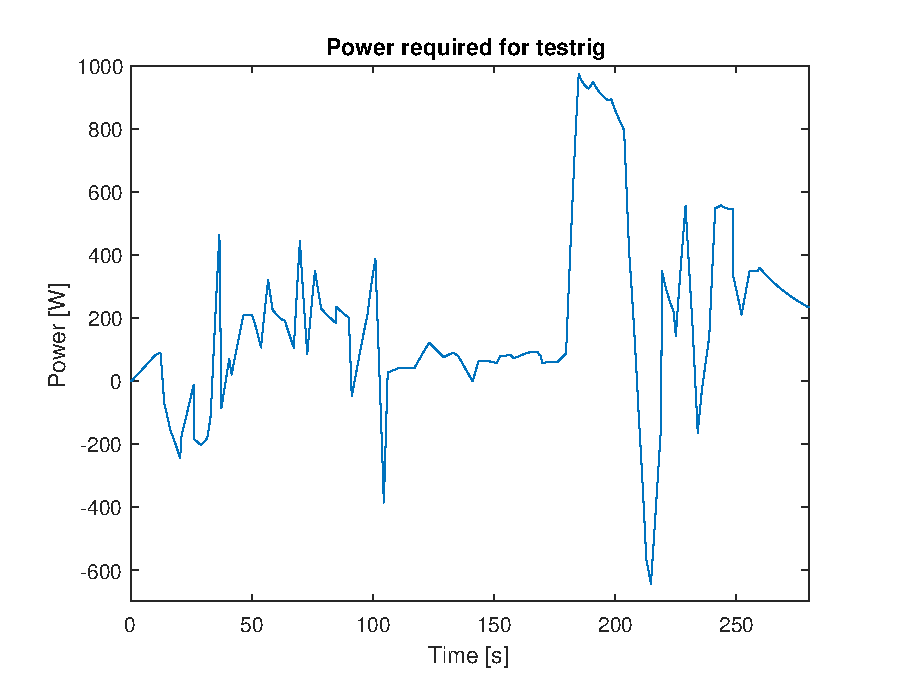
\includegraphics[width=0.5\textwidth]{./testrig/power_required_testrig.eps}
    \caption{Power required for the motor on the testrig.}
\end{figure}

\chapter{Discussion}
\section{Discussion}
\section{Conclusion}

\chapter{Future Work}
%\section{Futurework}

List of stuff to work on:

1. Separate ground between logic and power in testrig. Not possible because of the way we measure voltage. Should share logic ground with ESCON driver.

2. Map ICE.

3. Improve parameters of Elba in the plant model.

4. Local optimization? Not State flow.




% Bibliography
\bibliographystyle{plain}
\bibliography{mainbib}

\chapter*{Acknowledgments}
\addcontentsline{toc}{chapter}{Acknowledgments}
There have often been a sense of distance between students and the faculty in
many of the previous courses taken at KTH\@. During this project the feeling have
been the opposite, the mechatronics faculty have always been available and there
have been a real sense of unity between the teaching staff and the students in
the Eco Cars project. Our sincerest gratitude goes out to Mikael Hellgren for
your continuous support and guidance during the entire length of the project. We
would also like to thank Björn Möller for your belief in the project and allowing
the dialogue to be two sided. Our gratitude also goes out to Lei Feng for your
supervision of the project, ITRL for sponsoring and housing the project and SKF,
ECO2 and SHC for your sponsoring support. 

% This in not used atm
%\addtocontents{toc}{\protect\contentsline {part}{Appendices}{}{}}

\appendix
\part{Appendices}

%\chapter{Vehicle Stuff} \label{appA}
%\addtocontents{toc}{\protect\contentsline {part}{Appendices}{}{}}

\section{Vehicle Networks}
CAN is a controller area newtwork ref to can stuff blaha..

\chapter{Rig Calculations} \label{app:rigdata}
This appendix contains calculations made for the test rig dynamics model. 

\chapter{Elba 2015 report} \label{app:elba2015}
This appendix contains the report from the last iteration of Elba development.
Much of the information still holds true since most changes done this year are
improvements of existing systems.
\includepdf[pages={-}]{./appendices/Elba2015.pdf}


%% Append papers fore easy referencing, sota ice clutch
\part{Appended Papers}
\includepdf[pages=-]{appendices/MF2090_Report_VT16.pdf}
\includepdf[pages={1-17}]{appendices/Shell_Eco_Marathon_MachineDesign.pdf}
\end{document}
